\documentclass[a4paper, notitlepage, abstracton]{scrartcl}
\usepackage{geometry}
\usepackage[utf8]{inputenc}
\usepackage[italian]{babel}
\usepackage{fancyhdr}
\usepackage{lipsum}
\usepackage{float}

\usepackage{hyperref}
\usepackage{graphicx}
\usepackage{wrapfig}
\usepackage{listings}
\usepackage{float}
\usepackage{bytefield}
%\usepackage{fullpage}
\usepackage{algorithm}
\usepackage{algpseudocode}
\usepackage{amsmath}
\usepackage{todonotes}
\usepackage{tikz}

\newgeometry{top=3.5cm, left=2.5cm, right=2.5cm}
\usetikzlibrary{arrows,shapes}

\newcommand{\authorswe}{Davide Berardi, Matteo Martelli, Marco Melletti}

\pagestyle{fancy}
\rhead{Bajnarola}
\lhead{Progetto di sistemi distribuiti}

\rfoot{Davide Berardi, Matteo Martelli, Marco Melletti}
\lfoot{\thepage}
\cfoot{}
\renewcommand{\footrulewidth}{0.4pt}
\begin{document}

\title{Bajnarola}

\subtitle{Progetto di sistemi distribuiti}
\date{\today}

\pagenumbering{gobble}

\author{
	\begin{tabular}{c c c}
		Davide Berardi & Matteo Martelli & Marco Melletti\\
		0000712698     & 0000702472      & 0000699715
	\end{tabular}
}

\maketitle

\begin{abstract}
	In questo documento verrà descritto \emph{Bajnarola}, un videogame distribuito ispirato al gioco da tavolo \emph{Carcassonne}.
Saranno oggetto di questo documento le fasi di progettazione ed implementazione del sistema, con particolare riguardo per l'architettura di rete:
uno degli aspetti principali di un software interattivo multiutente distribuito.
Dopo aver introdotto il gioco e descritto gli aspetti progettuali ed implementativi, 
valuteremo il risultato ottenuto con le dovute considerazioni in termini di correttezza, usabilità ed affidabilità.

\end{abstract}

\pagenumbering{arabic}
\section{Introduzione}
Sempre più giochi da tavolo ormai vantano una versione digitale,
caratterizzata dalla possibilità di permettere agli utenti di giocare in
modalità multiplayer.
Allo stesso tempo però sono ancora rare implementazioni distribuite di
giochi multiplayer le quali spesso sono invece basate su un architettura
client server. In questo documento descriveremo il nostro lavoro di
progettazione ed implementazione della versione software di un gioco da
tavolo con particolare interesse riguardo l'architettura di rete
distribuita utilizzata nella modalità multiplayer.

\subsection{Carcassone}
In particolare è stato nostro interesse occuparci del remake del gioco
da tavolo Carcassonne. Quest'ultimo è un boardgame dei
primi anni 2000 basato su tessere che consiste nel creare un paesaggio medievale 
posizionando e accostando tra loro vari tipi di tessere, che rappresentano una parte di città, 
un tratto di strada, un campo o un monastero \footnote{Si fa riferimento
alla prima versione del gioco in cui non sono presenti fiumi, locande, ponti o altri elementi di paesaggio introdotti dalle varie espansioni}.
Completando più città, strade o monasteri attraverso tali tessere, i
giocatori (previsti da 2 a 5) accumulano i punti necessari a vincere la partita.
Al fine di comprendere al meglio le prossime sezione di questo documento, 
verra` illustrato di seguito il funzionamento del gioco.

All'inizio della partita, una specifica tessera è posizionata sul tavolo, scoperta; 
le altre tessere sono mescolate e rimangono coperte nel mazzo e mischiate.
Ciascuna di tali tessere rappresenta un frammento di paesaggio, e può contenere uno o più dei seguenti elementi:

\begin{itemize}
	\item tratti di strada, inclusi incroci e curve
    \item aree cittadine racchiuse da mura
    \item campi che circondano le città e accolgono le strade
    \item un monastero
\end{itemize}


\begin{figure}[H]
\centering
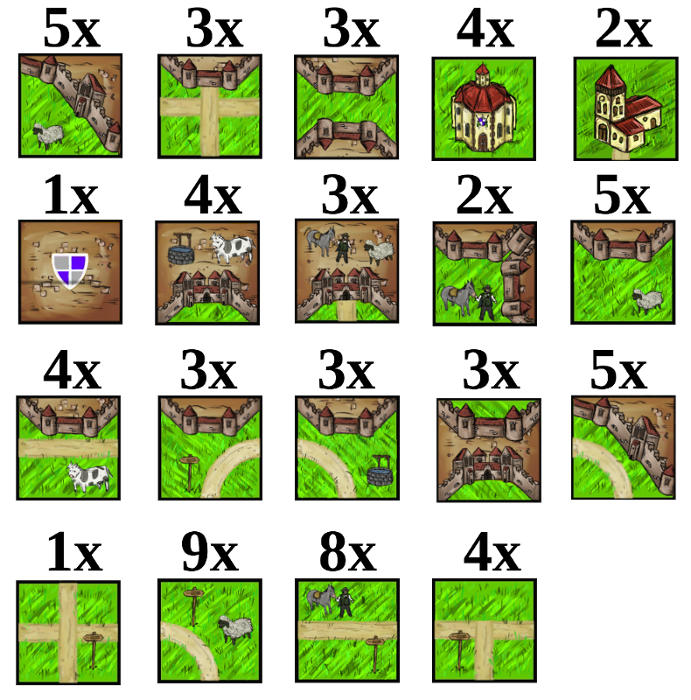
\includegraphics[width=\textwidth]{img/tiles.png}
\caption{Elenco delle tessere presenti nel gioco}
\label{img:tiles}
\end{figure}

A turno, un giocatore per volta estrae una tessera dal mazzo e la posiziona scoperta sul tavolo
a contatto con almeno una tessera già piazzata su uno o più lati, in modo da mantenere la coerenza con le vicine, 
estendendo eventuali strade, campi, o citta` già presenti.

Dopo aver posizionato la tessera, il giocatore può decidere di piazzare
una pedina detta \emph{meeple} su un elemento del paesaggio della tessera appena posizionata, reclamandone la proprietà a patto che non sia già stato reclamato da un altro giocatore.
Può accadere comunque che un elemento abbia più di un
proprietario se diviene una congiunzione di due elementi dello stesso
tipo non precedentemente adiacenti, in questo caso chi ha il numero maggiore di pedine sull'elemento rimane il proprietario, in caso di pareggio entrambi sono ritenuti proprietari e otterranno il punteggio relativo.

Quando un elemento viene completato, se ad esempio le mura di una città
vengono chiuse o se una strada ha due estremità chiuse, il proprietario
di quell'elemento acquisisce i relativi punti e tutte le pedine che erano su quell'elemento vengono restituite ai relativi proprietari. Il punteggio di un
elemento è dipendente dal numero e dal tipo di tessere che lo compongono.

Unica eccezione viene fatta per i poderi, che non vengono mai completati fino al termine della partita e sono soggetti ad un conteggio speciale.

Il gioco termina con il piazzamento dell'ultima tessera, al termine viene effettuato un conteggio finale dei punteggi derivanti dagli elementi non completati ma posseduti dai giocatori che avranno un valore differente in questa fase; vince il giocatore che, dopo il conteggio finale, ha totalizzato più punti.

Rimandiamo alla documentazione ufficiale di Carcassonne per ulteriori
dettagli.

La semplice struttura del gioco e la sua organizzazione a turni rende
interessante l'approccio distribuito in quanto si evita di incorrere in problemi 
di prestazioni tipici dei giochi reattivi. Questi ultimi infatti hanno requisiti prestazionali molto stringenti. In
particolare spesso richiedono che le comunicazioni di rete siano a bassa
latenza al fine di evitare
artefatti grafici fastidiosi dovuti ai ritardi di rete o all'overhead di
comunicazione.\\
Come già accennato, il gioco da noi considerato necessita invece di
requisiti prestazionali più laschi soprattuto per i lunghi tempi
decisionali degli utenti (comparati ai tempi di rete e computazionali).
\\
Vedremo nelle prossime sezioni i dettagli progettuali ed implementativi.
In ultimo forniremo una analisi valutativa dei risultati ottenuti dai test
con le dovute considerazioni finali.

\section{Aspetti progettuali}
Il gioco in questione è stato progettato nell'ottica di un sistema
resistente ai guasti, come richiesto da progetto.\\
L'aspetto critico studiato maggiormente per raggiungere tale
obiettivo è stato 
senz'altro la comunicazione, pensata per
risultare robusta e allo stesso tempo in grado di fornire reattività ai
client di gioco, nonostante quest'ultimo non utilizzi uno schema
realtime.

\subsection{Il gioco}
Le regole del gioco originale sono state vagamente semplificate per evitare eccessive complicazioni in fase di sviluppo, nello specifico abbiamo eliminato la meccanica dei poderi che avrebbe richiesto di strutturare dei meccanismi di valutazione complessi.

La logica del gioco e` divisa in due strati paralleli, quello ``fisico'' rappresentato dal tabellone che viene man mano creato e descrive la condizione esatta del tabellone di gioco e quello ``logico'' composto dagli elementi del paesaggio, che ne valuta lo stato ed informa lo strato fisico del completamento degli elementi.

I due strati agiscono quindi nelle due fasi del turno di un giocatore: il primo controlla che sia possibile piazzare la tessera pescata dove desidera il giocatore garantendo che non venga violata la continuita` del paesaggio, il secondo controlla la proprieta` dei vari elementi del paesaggio della tessera appena piazzata e permette o meno il piazzamento dei meeple, dopo di che` aggiorna i punteggi dei giocatori se rileva il completamento di un elemento di paesaggio.

Per valutare il completamento dei tre diversi elementi di paesaggio considerati vengono utilizzate tre tecniche specifiche:
\begin{description}
	\item[Monasteri] \hfill \\
		sono completi quando tutte le otto tessere adiacenti sono state piazzate, e` quindi sufficiente contare il numero dei vicini.
	\item[Strade] \hfill \\
		sono complete quando hanno incroci o citta` che le racchiudono, vengono contate quindi le tessere appartenenti alla strada che contengono un incrocio o una strada che finisce in una citta`, quando queste sono 2 l'elemento e` completo.
	\item[Città] \hfill \\
		sono complete quando tutto il muro di cinta e` chiuso, viene tenuto quindi il conto di quanti lati aperti sono rimasti su tutto il confine della citta`, quando questo numero scende a zero l'elemento e` completo.
\end{description}

\subsection{La comunicazione}
L'aspetto principale dell'intero sistema risulta l'architettura paritaria
dell'intera rete, questa e' stata progettata utilizzando una topologia token
ring, questo tipo di topologia fa in modo che il gioco possieda un
\textbf{ordine} tra i vari giocatori in base ad un tiro di dado come si farebbe
in una partita reale.\\
Come appena introdotto, la rete e' stata pensata come un \textbf{token ring}, il
problema di questo approccio pero' risulta nell'aggiornamento dello schema di
gioco; se la rete fosse completamente token ring i pacchetti dovrebbero
percorrere l'intero anello per giungere a tutti i giocatori, oppure aspettare
un intero turno di gioco per giungere al sistema di aggiornamento, complicando
inutilmente il sistema.\\
Per questi motivi e' stata scelta una topologia \textbf{completamente connessa}: anche se lo
schema di gioco non presenta particolari requisiti di latenza, ogni nodo
contattera' ogni volta il nodo possedente il turno, il quale terminata la sua
azione restituira' il controllo al nodo richiedente che potra' aggiornare il suo
stato locale.\\

\begin{figure}[H]
\begin{minipage}{.5\textwidth}
\centering
\begin{tikzpicture}[->,
	main node/.style={circle,draw,thick,fill=blue!20,minimum size=4mm},
	leader node/.style={circle,draw,thick,fill=green!20,minimum size=4mm}
]

	\def \n {5};
	\def \r {1.8cm};
	\def \m {8};

	\draw[->] (\m:\r) arc ({\m}:{360/\n -\m}:\r);

	\foreach \s in {2,...,\n} {
		\draw[->] ({360/\n * (\s-1) + \m}:\r) arc ({360/\n * (\s-1) + \m}:{360/\n * (\s) -\m}:\r);
		\node[main node] at ({360/\n * (\s-1)}:\r) {$\s$};
	}
	\node[leader node] at (0:\r) {1};
\end{tikzpicture}
\end{minipage}
\begin{minipage}{.5\textwidth}
\centering
\begin{tikzpicture}[->,
	main node/.style={circle,draw,thick,fill=blue!20,minimum size=4mm},
	leader node/.style={circle,draw,thick,fill=green!20,minimum size=4mm}
]

	\def \n {5};
	\def \r {1.8cm};
	\def \m {8};

	\draw[->,gray] (\m:\r) arc ({\m}:{360/\n -\m}:\r);

	\foreach \s in {2,...,\n} {
		\draw[->,gray] ({360/\n * (\s-1) + \m}:\r) arc ({360/\n * (\s-1) + \m}:{360/\n * (\s) -\m}:\r);
		\node[main node] at ({360/\n * (\s-1)}:\r) (\s) {$\s$};
	}
	\node[leader node] at (0:\r) (L) {1};

	\draw[->] (2) to[bend right=20] (L);
	\draw[->] (3) to[bend right=10] (L);
	\draw[->] (4) to[bend left=10] (L);
	\draw[->] (5) to[bend left=20] (L);
\end{tikzpicture}
\end{minipage}
\caption{\small{Tipologia token ring (sinistra) e tipologia completamente
connessa (destra).}}
\end{figure}
La tolleranza ai guasti di tipo crash e' quindi stata progettata in
quest'ottica, ogni nodo potra' accorgersi del crash di un altro giocatore
all'istante (o al momento dell'interrogazione), e riconfigurera' l'ordine
dell'anello di sorta.


\begin{figure}[H]
	\begin{minipage}{0.45\textwidth}
		\centering
		\begin{tikzpicture}[->,
			main node/.style={circle,draw,thick,fill=blue!20,minimum size=4mm},
			crashed node/.style={forbidden sign,draw,thick,fill=red!50,minimum size=4mm}
			]

			\def \n {5};
			\def \r {1.8cm};
			\def \m {8};

			\draw[->,gray] (\m:\r) arc ({\m}:{360/\n -\m}:\r);

			\foreach \s in {2,...,\n} {
				\draw[->,gray] ({360/\n * (\s-1) + \m}:\r) arc ({360/\n * (\s-1) + \m}:{360/\n * (\s) -\m}:\r);
				\node[main node] at ({360/\n * (\s-1)}:\r) (\s) {$\s$};
			}
			\node[crashed node] at (0:\r) (L) {1};

			\draw[->] (2) to[bend right=20] (L);
			\draw[->] (3) to[bend right=10] (L);
			\draw[->] (4) to[bend left=10] (L);
			\draw[->] (5) to[bend left=20] (L);
		\end{tikzpicture}
	\end{minipage}
	\begin{minipage}{0.45\textwidth}
		\centering
		\begin{tikzpicture}[->,
			main node/.style={circle,draw,thick,fill=blue!20,minimum size=4mm},
			crashed node/.style={circle,draw,thick,fill=gray,minimum size=4mm},
			leader node/.style={circle,draw,thick,fill=green!20,minimum size=4mm}
			]

			\def \n {5};
			\def \r {1.8cm};
			\def \m {8};


			\draw[->,gray] ({360/\n * (2-1) + \m}:\r) arc ({360/\n * (2-1) + \m}:{360/\n * (2) -\m}:\r);
			\node[leader node] at ({360/\n * (2-1)}:\r) (2) {$2$};
			\draw[->,gray] ({360/\n * (3-1) + \m}:\r) arc ({360/\n * (3-1) + \m}:{360/\n * (3) -\m}:\r);
			\node[main node] at ({360/\n * (3-1)}:\r) (3) {$3$};
			\draw[->,gray] ({360/\n * (4-1) + \m}:\r) arc ({360/\n * (4-1) + \m}:{360/\n * (4) -\m}:\r);
			\node[main node] at ({360/\n * (4-1)}:\r) (4) {$4$};
			\node[main node] at ({360/\n * (5-1)}:\r) (5) {$5$};

			\draw[->,gray] (5) to [bend right=50] (2);

			\node[crashed node] at (0:\r) (L) {1};
			\draw[->] (3) to[bend right=10] (2);
			\draw[->] (4) to[bend left=10] (2);
			\draw[->] (5) to[bend left=20] (2);
		\end{tikzpicture}
	\end{minipage}
	\caption{\small{Riconfigurazione dei client dovuta ad un crash}}
\end{figure}


\section{Aspetti implementativi}



\subsection{Il desing pattern MVC}
Il sistema \`e stato implementato utilizzando il design pattern \emph{MVC},
Model View Controller, questo design pattern aiuta lo sviluppo di applicazioni
``a camere stagne", separando il modello (la logica e il motore di gioco) dalla
grafica e dalla sua presentazione all'utente tramite un'entit\`a denominata
\textbf{controller}. Nello scenario del progetto questa entit\`a \`e stata
dotata della logica di gestione distribuita dello stato dei vari mondi di gioco.

\subsection{Implementazione dello schema di gioco}


In questo paragrafo vedremo brevemente l'implementazione dello schema e
della logica di gioco.
La figura \ref{img:model} mostra il diagramma delle classi del
componente \textbf{model} il quale racchiude tutte le funzionalità della logica
di gioco.\\
Come anticipato dalla fase progettuale, il model implementa i meccanismi che permettono
il collegamento logico delle tessere fra di loro, il rilevamento degli elementi completati
(città, strade, monasteri) e l'assegnamento dei punti ai loro rispettivi
proprietari.
\begin{figure}
\includegraphics[width=\textwidth]{img/modelClassDiagram.png}
\caption{Diagramma delle classi del modello di gioco}
\label{img:model}
\end{figure}

\subsection{L'interfaccia grafica}
L'interfaccia grafica (componente \textbf{view}) \`e basata sul motore Slick2D\footnote{\url{http://slick.ninjacave.com/}},  
questo mette a disposizione una libreria abbastanza semplice per realizzare interfacce grafice
anche complesse prive di rendering 3D.

L'intera esecuzione dell'inferfaccia grafica \`e affidata ad un thread dedicato, una
classe principale gestisce il dispatching degli aggiornamenti grafici e la lettura
dell'input.

Il motore di gioco lancia la funzione di rendering alla frequenza (\emph{refresh rate}) impostata, la classe principale
delega dunque la composizione della schermata alla classe che implementa scena attualmente visualizzata.
Parallelamente viene anche lanciata (con cadenza meno regolare) una funzione di aggiornamento (\texttt{void update()}) che interroga il controller e recupera nel thread della grafica gli eventuali aggiornamenti in coda (ad esempio tessere piazzate e punteggi segnati).

Alla stessa maniera, la gestione degli input viene passata alla scena corrente dalla classe principale in modo da interpretare le pressioni dei tasti e i movimenti del mouse nella maniera corretta.

\subsubsection{Interazione}
\begin{figure}[htbp]
	\includegraphics[width=\textwidth]{img/effects.jpg}
	\caption{Schermata di gioco}
	\label{img:game}
\end{figure}

In figura \ref{img:game} \`e mostrata una schermata di gioco, la parte centrale \`e occupata dal tavolo su cui vengono piazzate le tessere ed i meeple. 
Sui contorni della visuale di gioco vengono mostrati gli elementi dell'HUD (\emph{Heads-Up Display}): 
\begin{itemize}
\item in alto a sinistra i punteggi attuali dei partecipanti ancora in gioco;
\item in alto a destra compare un pulsante per attivare e disattivare lo zoom quando lo scenario eccede i limiti dell'HUD stesso, in questo caso si pu\`o spostare la visuale muovendo il puntatore verso i bordi della schermata oppure utilizando le frecce direzionali sulla tastiera;
\item in basso a sinistra i meeple ancora in mano al giocatore.
\end{itemize}
Inoltre se un giocatore \`e di turno l'HUD conterr\`a anche:
\begin{itemize}
\item in basso al centro il pulsante di confema del piazzamento;
\item in basso a destra la tessera da piazzare;
\item \emph{una volta confermato il piazzamento} (fig. \ref{img:gameMeeple}) sulla tessera da piazzare vengono evidenziate le posizioni su cui \`e possibile mettere un meeple (ammesso che il giocatore ne abbia ancora in mano).
\end{itemize}

Il giocatore di turno, spostando il mouse sui confini dello scenario creato, puo vedere un contorno nero che indica la possibilit\`a di tentare un piazzamento. Un click sinistro del mouse effettuer\`a il tentativo, mostrando la tessera in trasparenza se il piazzamento \`e possibile o un effetto rosso in caso contrario. 
Utilizzando la rotellina del mouse o il click destro \`e possibile ruotare la tessera.

\begin{figure}[htbp]
	\includegraphics[width=\textwidth]{img/meeplePlacement.jpg}
	\caption{Schermata di gioco: piazzamento meeple}
	\label{img:gameMeeple}
\end{figure}

Una volta confermato il piazzamento si pu\`o decidere di mettere un meeple su un elemento della tessera appena piazzata cliccando sul contorno del meeple e lo si pu\`o rimuovere cliccando sul meeple stesso.

Al termine di un turno ogni giocatore vedr\`a i risultati del piazzamento effettuato, gli elementi del territorio completati vengono evidenziati e, se qualche giocatore li possedeva, il punteggio dei singoli elementi viene mostrato sopra agli stessi, come anche il piazzamento o la restituzione dei meeple.

\subsection{La gestione e la distribuzione della rete}
	\subsubsection{Registrazione presso la lobby}
		Il primo passo svolto da ogni nodo di rete \`e la registrazione
		presso un server centralizzato comune, che implementa una o pi\`u
		``stanze" di gioco: le cosiddette lobby.\\
		Questo server aspetta la registrazione del numero
		specificato di partecipanti, inviando loro la lista dei
		giocatori per poi lasciargli il pieno controllo, chiudendo la stanza.

% TODO struttura pacchetti???
\begin{figure}[H]
\begin{minipage}[t]{0.45\textwidth}
\centering
\begin{tikzpicture}[->,
	main node/.style={circle,draw,thick,fill=green!20,minimum size=4mm},
	lobby node/.style={ellipse,draw,thick,fill=blue!20,minimum size=4mm}
]
	\node[lobby node] (L) {Lobby Server};

	\node[main node, below of=L,xshift=-18mm,yshift=-5mm] (1) {1};
	\node[main node, below of=L,xshift=-7mm,yshift=-10mm] (2) {2};
	\node[main node, below of=L,xshift=7mm, yshift=-10mm] (3) {3};
	\node[main node, below of=L,xshift=18mm,yshift=-5mm] (4) {4};

	\draw[->] (1) to[bend left=10] (L);
	\draw[->] (L) to[bend left=10] (1);

	\draw[->] (2) to[bend left=10] (L);
	\draw[->] (L) to[bend left=10] (2);

	\draw[->] (3) to[bend left=10] (L);
	\draw[->] (L) to[bend left=10] (3);

	\draw[->] (4) to[bend left=10] (L);
	\draw[->] (L) to[bend left=10] (4);
\end{tikzpicture}
\caption{\scriptsize Registrazione presso il server lobby}
\end{minipage}
\begin{minipage}[t]{0.45\textwidth}
\centering
\begin{tikzpicture}[->,
	main node/.style={circle,draw,thick,fill=green!20,minimum size=4mm},
	notacc node/.style={circle,draw,thick,fill=red!20,minimum size=4mm},
	lobby node/.style={ellipse,draw,thick,fill=blue!20,minimum size=4mm}
]
	\node[lobby node] (L) {Lobby Server};

	\node[main node, below of=L,xshift=-18mm,yshift=-5mm] (1) {1};
	\node[main node, below of=L,xshift=-7mm,yshift=-10mm] (2) {2};
	\node[main node, below of=L,xshift=7mm, yshift=-10mm] (3) {3};
	\node[main node, below of=L,xshift=18mm,yshift=-5mm] (4) {4};

	\node[notacc node,below of=L,yshift=-18mm] (5) {5};

	\draw[->] (5) to[bend left=10] (L);
	\draw[->] (L) to[bend left=10] (5);

\end{tikzpicture}
\caption{\scriptsize Eccezione del server alla richiesta di una lobby chiusa}
\end{minipage}
\end{figure}

\subsubsection{Lo schema con leader dinamico.}
Lo schema di distribuzione si basa sull'elezione di un leader ``dinamico", questo
leader \`e deciso in base ad un lancio di un dado iniziale (nella realta'
implementato come un random intero a 32 bit). Il
lancio viene distribuito tra i vari player, 
il giocatore con punteggio maggiore viene
quindi dichiarato come leader corrente, e da li a decrescere.
Inoltre il valore del tiro di dado del leader iniziale viene utilizzato da tutti i giocatori come seme per mescolare il mazzo di tessere, in modo da mantenere lo stato iniziale coerente.\\
La topologia risulta quindi una rete monodirezionale con passaggio del
testimone (token ring) per la decisione del leader corrente.


\subsubsection{Aggiornamenti allo stato}
	Uno degli aspetti pi\`u importanti del sistema di comunicazione del gioco
	\`e la presenza di classi di differenza (classe \textbf{TurnDiff}), le
	suddette classi rendono la comunicazione il pi\`u leggero possibile
	essendo composte da:\\

\begin{minipage}{.60\textwidth}
	\begin{itemize}
		\item Le coordinate della tessera posizionata;
		\item la rotazione della tessera posizionata;
		\item la posizione relativa del meeple se presente;
		\item il turno e il giocatore correnti.
	\end{itemize}
\end{minipage}
\begin{minipage}{.20\textwidth}
	\includegraphics{img/turndiff.png}
\end{minipage}

\subsubsection{Tolleranza ai guasti}
Il sistema risulta tollerante ai guasti di tipo \emph{crash}.
	Nel caso di un guasto di questo tipo sul nodo leader corrente, sar\`a il
	sistema ad invocare un'eccezione di tipo \textbf{RemoteException} verso
	i nodi interroganti, che lo elimineranno quindi dalla loro lista di
	interrogazione, riconfigurando l'anello.\\
	Nel caso di un guasto di un nodo intermedio il risultato sar\`a il
	medesimo al momento di un'interrogazione da parte dei vari nodi
	dell'anello (e.g. quando il nodo crashato sar\`a di turno).\\
	Questo genere di configurazione mantiene coerente lo stato locale delle
	diverse istanze, poich\`e ogni nodo aspetta la risoluzione delle varie
	mosse ad esso precedenti prima di essere interrogato a sua volta e poter
	agire.\\
	Questo schema \`e banalmente possibile utilizzando una semplice rete di
	tipo token ring, ma \`e stato scelto di implementare il tutto come una
	sorta di cricca per l'aggiornamento automatico e la visualizzazione dei
	risultati con latenze brevi: se si fosse ponderato per una struttura
	completamente circolare (utilizzante lo stesso modello logico) gli
	aggiornamenti allo stato locale sarebbero applicati solamente dopo che
	il controllo (e quindi la leadership) fosse tornata al nodo richiedente,
	risultando in un'attesa pari ad \textbf{N-1} turni. Essendo il gioco
	in questione un gioco di logica non propriamente reattivo e con turni
	di gioco potenzialmente molto lunghi e riflessivi, abbiamo optato
	per un modello pi\`u pesante da un punto di vista
	di scambio di informazioni, ma, allo stesso tempo, pi\`u reattivo per tutti i client.

	Le informazioni aggiuntive di numero di turno (clock logico) e nome del giocatore presenti nel diff vengono utilizzate insieme ad un id di gioco stabilito ad inizio partita per identificare alcuni problemi di consistenza: tutte le richeste verso il giocatore di turno specificano il clock e l'id della partita e vengono controllate da quest'ultimo prima di restituire il diff, allo stesso modo il diff deve contenere il nome del player che ha appena giocato e il clock logico del suo turno.
	Questo doppio controllo consente ai nodi di verificare con sufficiente confidenza che le informazioni contenute nel diff non siano frutto di un malfunzionamento e che i nodi richiedenti siano ancora sani.

\begin{figure}[H]
	\centering
	\includegraphics[width=\textwidth]{img/seq_diagram_play.png}
	\caption{Comunicazione in una partita d'esempio a 4 giocatori}
	\label{img:sequence}
\end{figure}

\subsubsection{Gestione della critical section}
	Il modello presenta una critical section ad ogni interrogazione di un leader
	(ogni nodo interrogante dovr\`a aspettare l'effettivo turno
	di gioco del leader), questa critical section \`e implementata come un
	\textbf{Lock} a barriera utilizzando la classe \textbf{ReentrantLock}.\\
	Ogni nodo verr\`a bloccato fino all'avvenuto piazzamento della tessera e
	alla relativa creazione della struttura \textbf{TurnDiff}.\\
	Questo modello di critical section locale non invalida il meccanismo di
	tolleranza ai guasti poich\`e se il processo leader subisce un
	\textbf{crash}, i vari richiedenti verranno liberati dalla critical
	section e gli verr\`a segnalato dal sistema di comunicazione il guasto.

\begin{figure}[H]
	\centering
	\includegraphics[width=\textwidth]{img/controllerClassDiagram.png}
	\caption{UML: Controller}
	\label{img:controller}
\end{figure}


\section{Valutazioni Finali e Conclusioni}
Al termine della fase di sviluppo abbiamo condotto diversi test al fine
di valutare l'esperienza di gioco.
In questa fase abbiamo appreso appieno l'importanza dell'utilizzo dei
design pattern e dell'accurata strutturazione gerarchica del modello delle
classi. In particolare il pattern MVC ci ha permesso di correggere
facilmente gli errori di implementazione.

Ci siamo concentrati sulla comprensione della correttezza del comportamento delle comunicazioni
tra i nodi della rete.

Dopo gli ultimi bugfix, non abbiamo più riscontrato problemi implementativi
nella fase finale di test e le interazioni fra i giocatori funzionano
come da aspettative. Inoltre l'esperienza di gioco risulta essere
particolarmente fluida e piacevole grazie alle ottimizzazioni introdotte
nell'interfaccia utente.

Per quanto riguarda l'affidabilità, la nostra implementazione è
tollerante ai guasti di tipo crash. La rete logica in Bajnarola infatti si
riorganizza automaticamente nel caso in cui uno o più nodi subiscano un
crash, permettendo agli utenti ancora in gioco di concludere la partita ed essere notificati dei guasti.\\

In conclusione tramite questo lavoro abbiamo avuto l'occasione di
approfondire il mondo dei sistemi distribuiti e allo stesso tempo
siamo riusciti a raggiungere un risultato implementativo molto
soddisfacente che verrà sicuramente arricchito da sviluppi futuri.


\end{document}
